\documentclass[conference]{IEEEtran}
\IEEEoverridecommandlockouts
% The preceding line is only needed to identify funding in the first footnote. If that is unneeded, please comment it out.
\usepackage{cite}
\usepackage{amsmath,amssymb,amsfonts}
\usepackage{algorithmic}
\usepackage{graphicx}
\usepackage{textcomp}
\usepackage{xcolor}
\def\BibTeX{{\rm B\kern-.05em{\sc i\kern-.025em b}\kern-.08em
    T\kern-.1667em\lower.7ex\hbox{E}\kern-.125emX}}
\begin{document}

\title{Feedback Assessment Two\\}

\author{\IEEEauthorblockN{George Lancaster}
\IEEEauthorblockA{\textit{dept. of Computer Science} \\
\textit{University of Bristol}\\
Bristol, United Kingdom \\
qv18258@bristol.ac.uk\\}}

\maketitle

\begin{abstract}
This document describes the concepts and motivation behind Cloud Chat, a cloud-based live-streaming and video chat service.
\end{abstract}
\begin{IEEEkeywords}
cloud, web-application, streaming, video chat, live.
\end{IEEEkeywords}
\section{Overview}
Cloud Chat will connect two clients, opening an audio and video stream between them. Data will be streamed to an AWS server, then back to the other chat participant. Users are not required to create an account to use the service, and will be invited to join a chat by email invitation only. AWS provides Simple Email Service, which can be used to automate the sending of invitations.
\par
Depending on time constraints, users may be able to create accounts and store a list of contact email addresses using S3 storage and Cognito. Although this is not the main focus of the project, it is a suitable extension, which allows users to create, read, update and delete data. 
\section{Motivation}
The motivation for this project is to show how a high-bandwidth, computationally expensive operation like video streaming can be performed seamlessly using cloud computation. Bi-directional video streaming involves two clients sending and receiving data simultaneously. By using cloud services, streaming speed will not be restricted by the server hardware, only by the bandwidth of the users. 
\par
Additionally, using a cloud provider for hosting allows for multiple video streams to be open concurrently without any interruption, or loss of quality to current streams. When a new stream is started, we can replicate the stream environment, and scale up the compute resources appropriately. In contrast, when a stream ends we can deallocate the compute resources and scale the application down. 
\par
Streaming requires the uninterrupted attention of one worker per connection to a stream, and workers are only released when the stream ends. This means that there can only be as many streams running at one time as there are workers. By using a cloud service, we are essentially using an unlimited number of workers, and therefore there is no upper limit on the number of simultaneous streams.
\section{Technical Challenges}
The greatest technical challenges are setting up the video streams between the two clients, and allowing for the system to scale with the number of current streams. Any problems encountered during development of the streams can be resolved by stream simulation. By sending and receiving a large amount of arbitrary data between clients, we can demonstrate that the service scales as expected.
\par
Whilst more time is required on the planning on the service, an initial investigation has found that it may be best to host the application using Docker, on Amazon Elastic Container Service (ECS) \cite{antonopoulos2010cloud}. By using Docker and ECS, each time a new stream is required, we can instantiate another chat image, which will automatically allocate more compute resources.
\par
Cloud Chat plans to build upon an existing open-source repository found on GitHub, which uses Flask and OpenCV to open and display a video stream from the webcam in the browser \cite{miguelgrinberg}. The repository has been released under the MIT license, and is therefore legal to use for this project. 
\begin{figure}[htbp]
\begin{center}
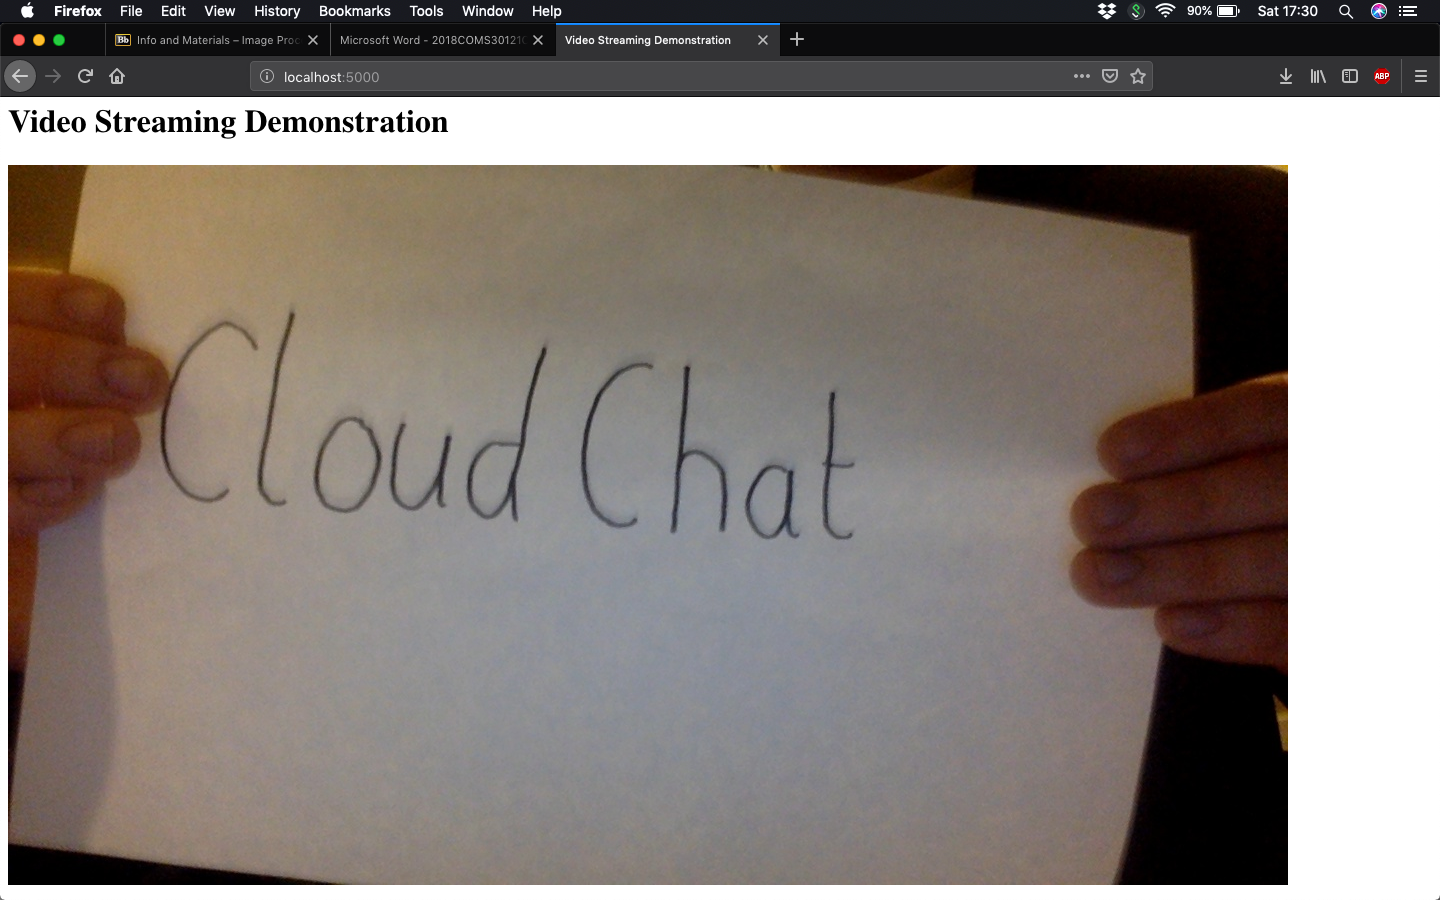
\includegraphics[width=0.6\linewidth]{screen.png}
\caption{Video stream captured using the open-source GitHub repository\cite{miguelgrinberg}.}
\label{default}
\end{center}
\end{figure}
\vspace{-0.5cm}
\section{Competitor Analysis}
Skype is conceptually similar to Cloud Chat, however it uses a network of nodes to connect clients in a peer-to-peer network \cite{baset2004analysis}. Cloud Chat will differ from Skype, in that data will first be streamed to the cloud server, before being sent to the recipient. Using the cloud ensures that there is a centralisation of control, rather than peers connecting to one another. 
\section{Conclusion}
The main goal of this project is to demonstrate how cloud services can be used to send and receive large amounts of live data between clients.

\bibliography{citations}
\bibliographystyle{unsrt}



\end{document}
